\documentclass[12pt,a4paper]{article}
\usepackage[utf8]{inputenc}
\usepackage[T1]{fontenc}
\usepackage{booktabs}
\usepackage{enumitem}
\title{Nek tenta grind}
\author{Yunshan Luo}


\renewcommand{\baselinestretch}{0.2}

\setlength{\hoffset}{-18pt}         
\setlength{\oddsidemargin}{0pt} % Marge gauche sur pages impaires
\setlength{\evensidemargin}{0pt} % Marge gauche sur pages paires
\setlength{\marginparwidth}{54pt} % Largeur de note dans la marge
\setlength{\textwidth}{481pt} % Largeur de la zone de texte (17cm)
\setlength{\voffset}{-18pt} % Bon pour DOS
\setlength{\marginparsep}{7pt} % Séparation de la marge
\setlength{\topmargin}{0pt} % Pas de marge en haut
\setlength{\headheight}{13pt} % Haut de page
\setlength{\headsep}{4pt} % Entre le haut de page et le texte
\setlength{\footskip}{27pt} % Bas de page + séparation
\setlength{\textheight}{720pt} % Hauteur de la zone de texte (25cm)

\usepackage{natbib}
\usepackage{graphicx}
\usepackage{amssymb}
\usepackage{amsmath} % Required for the align* environment
\usepackage{float}
\usepackage{pgfplots} 
\usepackage{algorithm}
\usepackage{algpseudocode} % test comment
\usepackage[hidelinks]{hyperref}
\pgfplotsset{compat=1.18}


\begin{document}
\section{Quiz 1}
\subsection{Produktionsgap}
\begin{itemize}
    \item $Y$ = faktisk BNP
    \item $Y^*$ = potentiell BNP
\end{itemize}
$
\text{Produktionsgap} = Y - Y^*
$

\subsection{Inflation, nominell och real ränta}
\begin{itemize}
    \item $\pi$ = inflation
    \item $R$ = nominell ränta
    \item $r$ = real ränta
    \item $P_t$ = prisnivå vid tidspunkt $t$
\end{itemize}
Vid tidspunkt $t$ kan jag köpa $\frac{x}{P_t}$ enheter av BNP. Om jag investerar pengarna med nominell ränta $R$, så kan jag vid tidspunkt $t+1$ köpa $\frac{x(1+R)}{P_{t+1}}$ enheter av BNP.

{\Large 
\[ 
r_{t+1} = \frac{\frac{x(1+R_t)}{P_{t+1}} - \frac{x}{P_t}}{\frac{x}{P_t}} =
\frac{1 + R_t}{1 + \pi_{t+1}}
\]
\[
r_{t+1} = \frac{1 + R_t}{1 + \pi_{t+1}} - 1
\]
}

\subsection{Real BNP tillväxt}
Använd ett år som basår t.ex år $n$ sedan för varje år beräkna:
\begin{gather*}
Q_{\text{år } 1} \cdot P_{n} \\
Q_{\text{år } 2} \cdot P_{n} \\
Q_{\text{år } 3} \cdot P_{n} \\
\vdots \\
Q_{\text{år } k} \cdot P_{n}
\end{gather*}
Ta sedan två år och beräkna tillväxten mellan dem

\subsection{AS-AD modellen}
\begin{figure}[H]
\centering
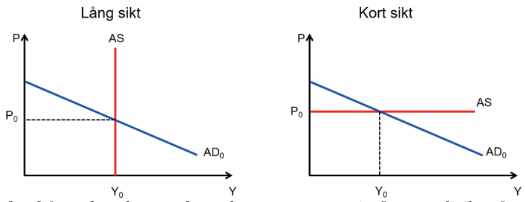
\includegraphics[width=1\textwidth]{AS-AD.png}
\end{figure}
\begin{itemize}
    \item \textbf{Långsikt: }Klassisk modell alla faktorer är fullt utnyttjade vertikal AS-kurva
    \begin{itemize}
        \item Y är oberoende av prisnivån
        \item Kapital stocken och humankapital är konstanta och fullt utnyttjade
    \end{itemize}
    \item \textbf{Kort sikt: }Keynsk modell horisontell AS-kurva 
    \begin{itemize}
        \item Priserna är fixa
        \item Y är beroende av prisnivån
    \end{itemize}
\end{itemize}

\subsection{Phillipskurva}
\begin{itemize}
    \item \textbf{x-axel: }Arbetslöshet
    \item \textbf{y-axel: }Inflation
\end{itemize}

\subsection{Identiteter}
\begin{itemize}
    \item \textbf{Y: }BNP
    \item \textbf{Q: }Import
    \item \textbf{C: }Privat konsumtion
    \item \textbf{I: }Investering
    \item \textbf{G: }Offentlig konsumtion
    \item \textbf{X: }Export
    \item \textbf{NX: }Nettoexport
    \item \textbf{TR: }Transfereringar
    \item \textbf{TA: }Skatters
    \item \textbf{BD: }Budgetunderskott
\end{itemize}
Nationalinkomstdentiteten:
\[
Y + Q = C + I + G + X 
\]
\[
Y = C + I + G + NX
\]
Disponibel inkomst:
\[
YD = Y + TR - TA
\]
Statens budgetunderskott:
\[
BD = G + TR - TA
\]
Sparande:
\[
S = I + BD + NX
\]

\section{Quiz 2}
\subsection{Ginikoefficienten}
\begin{figure}[H]
    \centering
    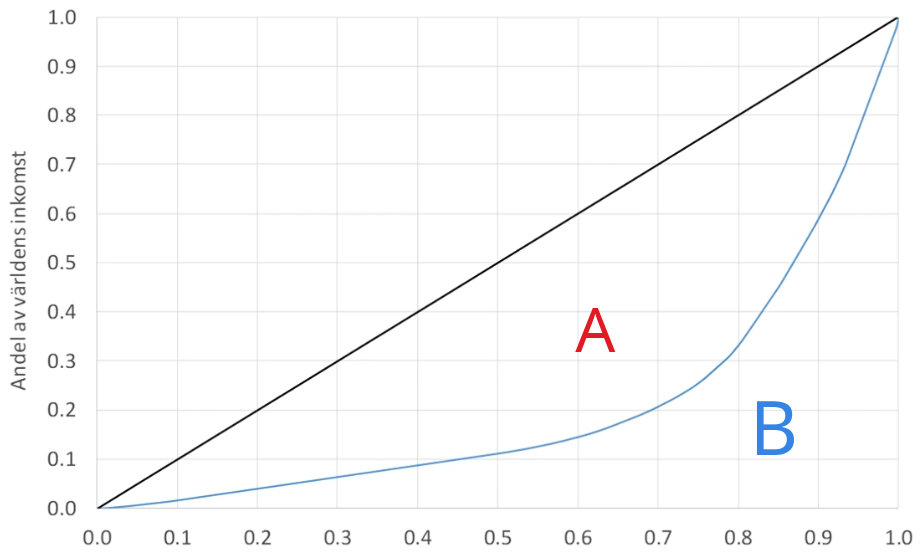
\includegraphics[width=0.75\textwidth]{lorenzkurvan.png}
\end{figure}
Ginikoefficienten: {\Large $\frac{A}{A+B}$}

\subsection{Solow modellen}
Antag att vi har en produktionsfunktion $Y=A\cdot F(K,N)$ där $N$ är arbetskraften och $K$ är kapitalstocken. I per capita termer blir det:
\begin{itemize}
    \item \textbf{Produktionsfunktionen per capita: }$y = f(k)$
    \item \textbf{Kapitalackumuleringsfuntion :}$\Delta k = sy -(d + n)k$
    \begin{itemize}
        \item $s$ = sparande kvot
        \item $d$ = kapitalförslitning
        \item $n$ = befolkningstillväxt
    \end{itemize}
    \item \textbf{Vid jämvikt: } $\Delta k = 0$
\end{itemize}

\subsection{Tillväxt dekomponering}
Antag att prodktionen ges av $Y = A \cdot K^{\alpha} \cdot N^{1-\alpha}$
\begin{enumerate}
    \item Dekomponera till: $\frac{\Delta Y}{Y} = \frac{\Delta A}{A} + \alpha \frac{\Delta K}{K} + (1-\alpha) \frac{\Delta N}{N}$
    \item Beräkna sedan varje term och returnera dem exempelvis teknologins tillväxt blir $\frac{\Delta A}{A}$
\end{enumerate}

\section{Quiz 3}
\subsection{Phillipskurvan}
Visar samband mellan inflation och arbetslöshet

\subsection{Kvantitetsteorin}
\begin{itemize}
    \item \textbf{Penningsmängd: }$M$
    \item \textbf{Pengars omsättningshastighet: }$V$
    \item \textbf{Prisnivå: }$P$
    \item \textbf{BNP: }$Y$
\end{itemize}
\[   
M \cdot V = P \cdot Y
\]

\subsection{Stagflation}
Hög inflation och hög arbetslöshet samtidigt

\subsection{Kapitalackumulering}
\[
\Delta K = sY - dK
\Delta k = sy - (d + n)k
\]
\begin{itemize}
    \item Kapitalackumulering: $\Delta K$
    \item Kapitalstocken per capita: $k$
    \item Sparande kvot: $s$
    \item Kapitalförslitning: $d$
    \item Befolkningstillväxt: $n$
    \item BNP per capita: $y$
\end{itemize}

\subsection{AS--AD förskjutning}
\begin{itemize}
    \item \textbf{x-axel: }Y = BNP
    \item \textbf{y-axel: }P = Prisnivå
    \item \textbf{AS: }Uppåtlutande
    \item \textbf{AD: }Nedåtlutande  
\end{itemize}

\section{Quiz 4}
\subsection{Friktionsarbetslöshet}
Arbetslösheten som existerar i jämnvikt då produktionen är lika med potentiell BNP

\subsection{Horizontell AS-kurva}
Extrem kort sikt är priser och löner helt fasta

\subsection{Vertikal AS-kurva}
Extrem lång sikt är alla faktorer rörliga och fullt utnyttjade

\subsection{Produktions händelser}
\begin{itemize}
    \item \textbf{Positiv efterfrågechock: }AD-kurvan skiftar åt höger
    \item \textbf{Negativ efterfrågechock: }AD-kurvan skiftar åt vänster
    \item \textbf{Positiv utbudschock: }AS-kurvan skiftar åt höger
    \item \textbf{Negativ utbudschock: }AS-kurvan skiftar åt vänster
\end{itemize}

\subsection{Arbetslöshet}
\begin{itemize}
    \item \textbf{p: }Sannolikheten att lämna sitt jobb
    \item \textbf{s: }Sannolikheten att hitta ett jobb
    \item \textbf{N: }Antal sysselsatta
    \item \textbf{U: }Antal arbetslösa
\end{itemize}
Den naturliga arbetslösheten ges av:
\[
u^* = \frac{p}{p+s}
\]

\noindent Jämnviktsflödet ges av:
\[
pN = sU
\]

\section{Quiz 5}
\subsection{Jämnvikts villkor}
\[
Y = C + I + G + NX
\]
\subsection{Konsumtionsfunktion med autonom konsumtion}
\[
C = C_0 + c \cdot YD
\]
\begin{itemize}
    \item \textbf{Autonom konsumtion: }$C_0$
    \item \textbf{Marginal konsumtionsbenägenhet: }$c$
    \item \textbf{Disponibel inkomst: }$YD$
    \item \textbf{Konsumtion: }$C$
\end{itemize}
\subsection{Disponibel inkomst}
\[
YD = (1+t)Y
\]
\begin{itemize}
    \item \textbf{BNP: }$Y$
    \item \textbf{Skattesats: }$t$
    \item \textbf{Disponibel inkomst: }$YD$
\end{itemize}

\subsection{Multiplikatorn}
\[
\alpha = \frac{\Delta Y}{\Delta G}
\]
\begin{itemize}
    \item \textbf{Multiplikatorn med skatt: }{\large $\alpha = \frac{1}{1 - c(1-t)}$}
    \item \textbf{Multiplikatorn utan skatt: }{\large $\alpha = \frac{1}{1 - c}$}
\end{itemize}

\section{Quiz 6}
\subsection{IS-LM modellen}
En graf med två kurvor:
\begin{itemize}
    \item \textbf{Y-axel: }R = ränta
    \item \textbf{X-axel: }Y = BNP
    \item \textbf{IS-kurvan: }Nedåtlutande
    \item \textbf{LM-kurvan: }Uppåtlutande
\end{itemize}

Kurvskiften i IS-LM modellen:
\begin{itemize}
    \item \textbf{Positiv efterfrågechock: }IS-kurvan skiftar åt höger
    \item \textbf{Negativ efterfrågechock: }IS-kurvan skiftar åt vänster
    \item \textbf{Positiv penningmängdschock: }LM-kurvan skiftar åt höger
    \item \textbf{Negativ penningmängdschock: }LM-kurvan skiftar åt vänster
\end{itemize}

\subsection{Omskrivning med AD-AS}
Hitta IS-kurvan i AD-AS modellen:
\begin{enumerate}
    \item $AD = C + I + G + NX$
    \item Lös $Y = AD$
    \item Lös ut $Y$ som en funktion av $i$
    \item Där fås IS-kurvan
\end{enumerate}

Hitta LM-kurvan i AD-AS modellen:
\begin{enumerate}
    \item $LM = M/P$
    \item Lös $M/P = L(Y, i)$
    \item Lös ut $i$ som en funktion av $Y$
    \item Där fås LM-kurvan
\end{enumerate}


\subsection{Kryssfrågor}
\begin{enumerate}[label=\arabic*.]
    
    % Document 1
    \item Vilket av följande alternativ visar den fundamentala nationalinkomstidentiteten?
    \begin{enumerate}[label=\alph*)]
        \item $Y - Q = C + I + G + X$
        \item $Y - Q = C + I + G - X$
        \item $Y + Q = C + I + G + X$
        \item $Y + Q = C + I + G - X$
        \item $Y + X = C + I + G + NX$
    \end{enumerate}

    \item Hur hög (med exakt uträkning) är den reala räntan i procent om den nominella räntan är 7 procent och inflationen är 5 procent?
    \begin{enumerate}[label=\alph*)]
        \item $r = 100 \times \frac{0.02}{1.07}$
        \item $r = 100 \times \frac{0.07}{1.02}$
        \item $r = 100 \times \frac{0.02}{1.05}$
        \item $r = 100 \times \frac{0.05}{1.05 \times 1.07}$
        \item Inget av ovanstående alternativ är korrekt.
    \end{enumerate}

    \item Antag att landet enbart tillverkar två varor, vara A och vara B och att vi har följande pris- och kvantitetsstatistik för år 1 och år 2. Baserat på statistiken i tabellen och avrundat till en decimal, hur hög är inflationen mätt med BNP-deflatorn om vi låter år 2 utgöra basår?
    
    \begin{tabular}{lcc}
        \toprule
         & \textbf{År 1} & \textbf{År 2} \\
        \midrule
        \textbf{Pris} & & \\
        Vara A & 50 & 54 \\
        Vara B & 125 & 120 \\
        \midrule
        \textbf{Kvantitet} & & \\
        Vara A & 400 & 410 \\
        Vara B & 30 & 45 \\
        \bottomrule
    \end{tabular}
    
    \begin{enumerate}[label=\alph*)]
        \item 5.4\%
        \item 5.8\%
        \item 6.1\%
        \item 9.3\%
        \item Inget av ovanstående alternativ är korrekt.
    \end{enumerate}

    \item \textit{[Figure shows Inflationsförändring i procentenheter on y-axis and Arbetslöshet i procent on x-axis]} Vad kallas kurvan som visas i figuren?
    \begin{enumerate}[label=\alph*)]
        \item Phillipskurva
        \item Beveridgekurva
        \item Lorentzkurva
        \item Lafferkurva
        \item Engelkurva
    \end{enumerate}

    \item Vad definierar en konjunkturåterhämtning?
    \begin{enumerate}[label=\alph*)]
        \item Ett positivt och stigande produktionsgap.
        \item Ett positivt men minskande produktionsgap.
        \item Ett negativt men stigande produktionsgap.
        \item Ett negativt och minskande produktionsgap.
        \item Deflation och ökad arbetslöshet.
    \end{enumerate}

    \item Vilken är en lämplig åtgärd från en oberoende centralbank om inflationstakten oväntat och kraftigt understiger inflationsmålet?
    \begin{enumerate}[label=\alph*)]
        \item Driva en kontraktiv penningpolitik.
        \item Försöka höja räntan i ekonomin.
        \item Påverka penningmängden genom att sälja statsobligationer.
        \item Påverka penningmängden genom att köpa statsobligationer.
        \item Driva en åtstramande finanspolitik.
    \end{enumerate}

    \item Vad är en Taylorregel?
    \begin{enumerate}[label=\alph*)]
        \item Den visar hur finanspolitiken bör utformas baserat på rådande arbetslöshet.
        \item Den visar hur finanspolitiken bör utformas baserat på rådande produktionsgap.
        \item Den visar hur den aggregerade efterfrågan i ekonomin i genomsnitt påverkas av förändringar i finanspolitiken.
        \item Den hjälper regeringen att bestämma ramarna för de finanspolitiska utgifterna baserat på rådande ekonomiska förhållanden.
        \item Den hjälper centralbanken att bestämma sin målränta baserat på rådande ekonomiska förhållanden.
    \end{enumerate}

    \item Antag en enkel modell utan en offentlig sektor och att en ökning av de autonoma investeringarna med 6 miljoner kronor leder till en ökning av jämviktskonsumtionen med 14 miljoner kronor. Hur stor är den marginella sparbenägenheten?
    \begin{enumerate}[label=\alph*)]
        \item 0.1
        \item 0.2
        \item 0.3
        \item 0.7
        \item Inget av ovanstående alternativ är korrekt.
    \end{enumerate}

    \item \textit{[Figure shows Vakanser i procent av arbetskraften on y-axis and Arbetslöshet i procent av arbetskraften on x-axis]} Vad kallas kurvan i figuren?
    \begin{enumerate}[label=\alph*)]
        \item Phillipskurva.
        \item Lorentzkurva.
        \item Engelkurva.
        \item Lafferkurva.
        \item Beveridgekurva.
    \end{enumerate}

    \item Antag att BNP i landet kan beskrivas av ekvationen $Y = K^{0.5}$ där Y står för BNP och K för den aggregerade kapitalstocken. Kapitalackumuleringsfunktionen ges i sin tur av $\Delta K = 0.2Y - 0.05K$ där $\Delta K$ står för förändring av kapitalstocken. Hur hög är ekonomins långsiktiga tillväxttakt?
    \begin{enumerate}[label=\alph*)]
        \item 0 procent.
        \item 2 procent.
        \item 4 procent.
        \item 5 procent.
        \item Inget av ovanstående alternativ är korrekt.
    \end{enumerate}

    % Document 2
    \item Vad skiljer BNP-deflatorn och konsumentprisindex (KPI) åt?
    \begin{enumerate}[label=\Alph*.]
        \item KPI inkluderar fler varor än BNP-deflatorn.
        \item BNP-deflatorn baseras på en fast varukorg medan KPI inte gör det.
        \item BNP-deflatorn inkluderar inte tjänster medan KPI gör det.
        \item KPI inkluderar färre varor än BNP-deflatorn.
        \item BNP-deflatorn inkluderar importerade varor medan KPI inte gör det.
    \end{enumerate}

    \item Phillipskurvan visar ett samband mellan,
    \begin{enumerate}[label=\Alph*.]
        \item Jobbvakanser och arbetslöshet.
        \item Arbetslöshet och inflation.
        \item Inflation och BNP.
        \item Produktionsgap och real ränta.
        \item Arbetslöshet och BNP.
    \end{enumerate}

    \item Vad menas med friktionsarbetslöshet?
    \begin{enumerate}[label=\Alph*.]
        \item Det är den arbetslöshet som råder då produktionsgapet är lika med noll.
        \item Det är den arbetslöshet som uppstår till följd av en utbudschock.
        \item Det är den arbetslöshet som orsakas av lagstadgade minimilöner.
        \item Det är motsatsen till den så kallade naturliga arbetslösheten.
        \item Det är den arbetslöshet som uppstår på grund av så kallade skoläderkostnader.
    \end{enumerate}

    \item Beveridgekurvan visar ett samband mellan,
    \begin{enumerate}[label=\Alph*.]
        \item BNP och arbetslöshetsgrad.
        \item Arbetslöshetsgrad och arbetslöshetens längd.
        \item Vakansgrad och arbetskraftsdeltagande.
        \item Arbetslöshetsgrad och vakansgrad.
        \item Tillväxt och arbetslöshetsgrad.
    \end{enumerate}

    \item I den långsiktiga AD-AS-modellen gäller att...
    \begin{enumerate}[label=\Alph*.]
        \item ...penningpolitik kan påverka prisnivån, men inte produktionsvolymen.
        \item ...penningpolitik kan påverka produktionsvolymen, men inte prisnivån.
        \item ...finanspolitik, men inte penningpolitik, kan påverka både produktionsvolymen och prisnivån.
        \item ...penningpolitik, men inte finanspolitik, kan påverka både produktionsvolymen och prisnivån.
        \item ...varken finanspolitik eller penningpolitik kan påverka prisnivån.
    \end{enumerate}

    \item Varför kan det vara bra att ha en viss positiv inflation jämfört med en konstant prisnivå?
    \begin{enumerate}[label=\Alph*.]
        \item Det minskar risken för stagflation.
        \item Det minskar risken för hysteresis.
        \item Det minskar såväl meny- som skoläderkostnader.
        \item En reallönesänkning kan då ske utan att det kräver minskade nominella löner.
        \item Inget av ovanstående alternativ är korrekt.
    \end{enumerate}

    \item Antag en modell utan utrikeshandel och utan offentlig sektor och där investeringarna är oberoende av räntenivån. Hur hög är multiplikatorn om en ökning av de autonoma investeringarna med 100 kronor leder till en ökning av jämviktskonsumtionen med 400 kronor?
    \begin{enumerate}[label=\Alph*.]
        \item 1,0.
        \item 2,0.
        \item 3,0.
        \item 4,0.
        \item 5,0.
    \end{enumerate}

    \item LM-kurvan visar...
    \begin{enumerate}[label=\Alph*.]
        \item ...kombinationer av inflation och nominell ränta när det råder full sysselsättning.
        \item ...sambandet mellan produktionsgap och nominell ränta.
        \item ...kombinationer av arbetslöshetsgrad och vakansgrad då det råder full sysselsättning.
        \item ...kombinationer av ränta och inkomst där det råder jämvikt på varumarknaden.
        \item ...kombinationer av ränta och produktionsnivåer där efterfrågan på pengar motsvarar utbudet av pengar.
    \end{enumerate}

    \item Antag att ett lands totala sparande är 400 kronor samtidigt som investeringarna är 80 kronor och nettoexporten är 140 kronor. Hur stort är det offentliga budgetunderskottet?
    \begin{enumerate}[label=\Alph*.]
        \item -340 kronor.
        \item 180 kronor.
        \item 340 kronor.
        \item 460 kronor.
        \item 620 kronor.
    \end{enumerate}

    \item Om inflationen är lägre än förväntat kommer det att...
    \begin{enumerate}[label=\Alph*.]
        \item ...gynna låntagarna på långivarnas bekostnad.
        \item ...gynna långivarna på låntagarnas bekostnad.
        \item ...gynna både låntagare och långivare.
        \item ...missgynna både låntagare och långivare.
        \item Inget av ovanstående alternativ är korrekt.
    \end{enumerate}

    % Document 3
    \item Vilket av följande påståenden är korrekt?
    \begin{enumerate}[label=\Alph*.]
        \item Den Keynesianska utbudskurvan är mest relevant för långsiktig analys medan den klassiska utbudskurvan är mest relevant för kortsiktig analys.
        \item Den Keynesianska utbudskurvan är mest relevant för kortsiktig analys medan den klassiska utbudskurvan är mest relevant för långsiktig analys.
        \item Den Keynesianska utbudskurvan är lämpligt att använda för att visa hur skiften i efterfrågekurvan påverkar ekonomin på medellång sikt.
        \item Den klassiska utbudskurvan är lämpligt att använda för att visa hur skiften i efterfrågekurvan påverkar ekonomin på medellång sikt.
        \item Enligt den Keynesianska utbudskurvan kommer en ökad offentlig konsumtion att leda till en ökad naturlig arbetslöshet.
    \end{enumerate}

    \item Enligt Eurostat har vi följande uppgifter för Sverige år 2023, allt uttryckt i miljarder Euro: BNP 541, Privat konsumtion 243, Investeringar 135, Offentlig konsumtion 142, Export 298. Hur stor import hade Sverige 2023 mätt i miljarder Euro?
    \begin{enumerate}[label=\Alph*.]
        \item 21.
        \item 277.
        \item 319.
        \item 1095.
        \item Inget av ovanstående svarsalternativ är korrekt.
    \end{enumerate}

    \item Om inflationen ligger under målet på 2 procent, vad kan Riksbanken göra för att höja inflationen?
    \begin{enumerate}[label=\Alph*.]
        \item Sälja statsobligationer.
        \item Höja styrräntan.
        \item Köpa statsobligationer.
        \item Minska köpkraften i ekonomin.
        \item Riksbanken kan inte göra någonting för att höja inflationen i ekonomin. De kan bara agera för att sänka en för hög inflation.
    \end{enumerate}

    \item Antag att prisnivån ökar och BNP minskar på medellång sikt. Vilket svarsalternativ är förenligt med det scenariot?
    \begin{enumerate}[label=\Alph*.]
        \item Den aggregerade efterfrågekurvan har skiftat åt vänster.
        \item Den aggregerade efterfrågekurvan har skiftat åt höger.
        \item Den aggregerade utbudskurvan har skiftat åt vänster.
        \item Den aggregerade utbudskurvan har skiftat åt höger.
        \item Den aggregerade efterfrågekurvan och den aggregerade utbudskurvan har båda skiftat åt höger.
    \end{enumerate}

    \item Vad kallas en situation där det samtidigt råder en hög arbetslöshet och en hög inflation?
    \begin{enumerate}[label=\Alph*.]
        \item Dynamic scoring.
        \item Employment instability.
        \item Konjunkturuppgång.
        \item Hysteresis.
        \item Stagflation.
    \end{enumerate}

    \item Antag att ekonomins BNP fås av produktionsfunktionen $Y = A K^{0.3} N^{0.7}$. Hur hög är teknologins tillväxttakt (uträknad som en Solowresidual) om vi vet att BNP ($Y$) vuxit med 10 procent samtidigt som kapitalstocken ($K$) vuxit med 5 procent och populationen ($N$) med 4 procent?
    \begin{enumerate}[label=\Alph*.]
        \item 0,5 procent.
        \item 1,0 procent.
        \item 2,2 procent.
        \item 5,7 procent.
        \item 8,8 procent.
    \end{enumerate}

    \item En förbättrad matchning mellan arbetssökanden och lediga jobb på arbetsmarknaden innebär att:
    \begin{enumerate}[label=\Alph*.]
        \item vi rör oss åt höger utmed en given Beveridgekurva.
        \item vi rör oss åt vänster utmed en given Beveridgekurva.
        \item Beverdigekurvan skiftar inåt mot origo.
        \item Beveridgekurvan skiftar utåt bort från origo.
        \item den kortsiktiga Phillipskurvan skiftar uppåt.
    \end{enumerate}

    \item Den så kallade kvantitetsteorin beskriver ett samband mellan den nominella penningmängden (M), prisnivån (P), BNP (Y) och pengars omsättningshastighet (V). Vilket svarsalternativ beskriver hur det sambandet ser ut?
    \begin{enumerate}[label=\Alph*.]
        \item $P \times V = M \times Y$
        \item $P \times M = V \times Y$
        \item $Y / V = M \times P$
        \item $V \times M = P \times Y$
        \item Inget av ovanstående svarsalternativ är korrekt.
    \end{enumerate}

    \item BNP-deflatorn och producentprisindex (PPI) skiljer sig åt eftersom,
    \begin{enumerate}[label=\Alph*.]
        \item BNP-deflatorn inkluderar importerade varor medan PPI inte gör det.
        \item PPI inkluderar fler varor än BNP-deflatorn.
        \item BNP-deflatorn inkluderar inte tjänster medan PPI gör det.
        \item BNP-deflatorn mäter inflationsförändringar tidigare än PPI.
        \item PPI baseras på en given korg med varor/tjänster medan BNP-deflatorn inte gör det.
    \end{enumerate}

    \item Om inflationen är lägre än förväntat kommer det att:
    \begin{enumerate}[label=\Alph*.]
        \item missgynna både låntagare och långivare.
        \item gynna både låntagare och långivare.
        \item gynna långivarna på låntagarnas bekostnad.
        \item gynna låntagarna på långivarnas bekostnad.
        \item leda till att köpkraften i ekonomin minskar mer än förväntat.
    \end{enumerate}

    % Document 4
    \item Vilket av följande påstående avseende tillväxtmodeller är korrekt?
    \begin{enumerate}[label=\Alph*.]
        \item Solowmodellen har tilltagande marginalavkastning på kapital.
        \item AK-modellen har tilltagande marginalavkastning på kapital.
        \item Den långsiktiga tillväxttakten är exogen i Solowmodellen.
        \item AK-modellen uppfyller Inadavillkoren.
        \item Den långsiktiga tillväxttakten är exogen i AK-modellen.
    \end{enumerate}

    \item \textit{[Figure shows Inflation i procent on y-axis and Arbetslöshet i procent on x-axis]} Vad kallas kurvan i figuren?
    \begin{enumerate}[label=\Alph*.]
        \item Phillipskurva.
        \item Okuns lag.
        \item Beveridgekurva.
        \item IS-kurva.
        \item LM-kurva.
    \end{enumerate}

    \item På 1970-talet upplevde Sverige en situation som kallas för stagflation. Vad betyder det?
    \begin{enumerate}[label=\Alph*.]
        \item Hög arbetslöshet tillsammans med en hög inflation.
        \item Extremt låg arbetslöshet tillsammans med en extremt hög inflation.
        \item Låg arbetslöshet tillsammans med en negativ inflation.
        \item Hög arbetslöshet tillsammans med en negativ inflation.
        \item Kraftiga statliga budgetöverskott tillsammans med en hög inflation.
    \end{enumerate}

    \item Konsumentprisindex var 207,8 år 1990 och 403,7 år 2023. Hur många procent ökade konsumentpriserna per år i genomsnitt under perioden?
    \begin{enumerate}[label=\Alph*.]
        \item Cirka 1,2 procent.
        \item Cirka 1,8 procent.
        \item Cirka 2,0 procent.
        \item Cirka 3,5 procent.
        \item Cirka 4,2 procent.
    \end{enumerate}

    \item Antag att Sveriges konsumtionsfunktion ges av $C = 400 + 0,8YD$, där C står för konsumtion och YD för disponibel inkomst. Hur hög är multiplikatorn om vi antar att landet saknar en offentlig sektor?
    \begin{enumerate}[label=\Alph*.]
        \item 0,80.
        \item 1,25.
        \item 2,25.
        \item 5,00.
        \item Inget av ovanstående alternativ är korrekt.
    \end{enumerate}

    \item Vilket av följande påståenden är korrekt?
    \begin{enumerate}[label=\Alph*.]
        \item Förändringar i real BNP inkluderar både kvantitet- och prisförändringar.
        \item Förändringar i nominell BNP inkluderar kvantitetsförändringar, men inte prisförändringar.
        \item BNP-deflatorn definieras som real BNP dividerat med nominell BNP.
        \item BNP-deflatorn definieras som real BNP multiplicerat med nominell BNP.
        \item BNP-deflatorn definieras som nominell BNP dividerat med real BNP.
    \end{enumerate}

    \item Vilket av följande svarsalternativ visar den fundamentala nationalinkomstidentiteten?
    \begin{enumerate}[label=\Alph*.]
        \item $Y + Q = C + I + G - X$
        \item $Y + Q = C + I + G + X$
        \item $Y + TR - TA = C + I + G + NX$
        \item $Y + NX = C + I + G$
        \item $Y = BD + I$
    \end{enumerate}

    \item Vilket av följande påståenden är korrekt om vi har en AS-AD-modell med en klassisk aggregerad utbudskurva?
    \begin{enumerate}[label=\Alph*.]
        \item Lönerna är orörliga.
        \item Arbetslösheten befinner sig alltid vid sin naturliga nivå.
        \item En expansiv finanspolitik ökar BNP.
        \item Prisnivån påverkas inte av förändringar i efterfrågan.
        \item Inget av ovanstående alternativ är korrekt.
    \end{enumerate}

    \item Hur stora är landets investeringar om sparandet är 1000 kronor, nettoexporten 200 kronor och det offentliga budgetunderskottet 450 kronor?
    \begin{enumerate}[label=\Alph*.]
        \item 350 kronor.
        \item 350 kronor.
        \item 750 kronor.
        \item 350 kronor.
        \item Inget av ovanstående svarsalternativ är korrekt.
    \end{enumerate}

    \item När ekonomin går in i en lågkonjunktur kan vi förvänta oss att,
    \begin{enumerate}[label=\Alph*.]
        \item Inflationen och arbetslösheten ökar.
        \item Inflationen och produktionen ökar.
        \item Inflationen minskar och arbetslösheten ökar.
        \item Inflationen minskar och produktionen ökar.
        \item Inget av ovanstående alternativ är korrekt.
    \end{enumerate}

\end{enumerate}

\newpage
\section*{Answers}

\begin{enumerate}[label=\arabic*.]
    \item c
    \item c
    \item c
    \item a
    \item c
    \item d
    \item e
    \item d
    \item e
    \item a
    \item D
    \item B
    \item A
    \item D
    \item A
    \item D
    \item E
    \item E
    \item B
    \item B
    \item B
    \item B
    \item C
    \item C
    \item E
    \item D
    \item C
    \item D
    \item E
    \item C
    \item C
    \item A
    \item A
    \item C
    \item D
    \item E
    \item B
    \item B
    \item A
    \item C
\end{enumerate}

\end{document}












\end{document}
